\section{Bereitstellen der Infrastruktur} \label{sec:infra}
Zu Beginn wird die Infrastruktur basierend auf dem theoretisch erarbeiteten Konzept in Azure bereitgestellt. Das Vorgehen und notwendige Entscheidungen bezüglich der Ressourcenkonfiguration, die sich nicht aus den Anforderungen ableiten lassen, orientieren sich an bestehender Literatur und Dokumentation.

\subsection{Ressourcenverwaltung mit Infrastructure-As-Code} \label{subsec:infra:konfig:iac}
In Azure müssen alle Ressourcen genau einem Container zugeordnet werden, der sogenannten Ressourcengruppe. Über diese können ein gemeinsamer Lebenszyklus, Berechtigungen und Richtlinien geteilt werden \cite{rendon_deploy_2022}. Für die Ressourcen des BI~=Systems wird eine Ressourcengruppe in der Region West-Europa erstellt. Dieser Standort wird für alle Ressourcen in diesem Prototyp übernommen.

Die benötigten Ressourcen können über einen Webbrowser im Azure Portal erstellt und verwaltet werden \cite{chilberto_building_2020}. Zum Erstellen einer komplexeren Architektur ist jedoch der \ac{arm} besser geeignet. Damit können beliebige Azure Komponenten flexibel über parametrisierbare Templates im JSON-Format, erstellt und verwaltet werden. Das macht \ac{arm} weniger fehleranfällig und zeitsparender als die Konfiguration aller einzelnen Komponenten über das Azure Portal \cite{monadjemi_azure-administration_2017}. Aus den genannten Gründen soll ein ARM~=Template erstellt werden, um das Cloud BI~=System bereitzustellen. Zusätzlich ermöglicht der \textit{Infrastructure-As-Code} Ansatz die Anwendung von \textit{DevOps}. Das bedeutet, dass die ARM-Templates in einer Versionskontrolle verwaltet werden und die Infrastruktur darüber automatisiert bereitgestellt werden kann. Dadurch kann auch die Verwaltung von mehreren Umgebungen (üblicherweise Entwicklung, Test und Produktion) vereinfacht werden \cite{riscutia_data_2021}. Für den DevOps Prozess wird die Plattform GitHub verwendet. Hier wird ein GitHub Actions Workflow erstellt, der automatisch ausgeführt wird, wenn ein neuer Commit hochgeladen wird und dann die Bereitstellung der Ressourcen übernimmt. Der Workflow wird in einer YAML-Datei definiert. Der Inhalt wurde aus \citetitle{rendon_deploy_2022} übernommen und besteht aus zwei Aktionen. Zunächst wird ein Login ausgeführt, bevor anschließend das ARM-Template in Azure bereitgestellt wird. Damit diese beiden Aktionen möglich sind, wird im \ac{aad} ein \textit{service principal} erstellt, der die notwendigen Rechte hat, um Ressourcen zu verändern. Die Zugansdaten für den \textit{service principal} werden in GitHub als verschlüsselte Umgebungsvariable hinterlegt. Das gilt auch für weitere Parameter, wie den Namen der Ressourcengruppe oder geheim zuhaltende Parameter wie Passwörter \cite[vgl.][]{rendon_deploy_2022}. Da das \ac{arm}-Template umfangreich ist und im Prinzip nur eine Auflistung von Definitionen und Parametern der Ressourcen ist, wird es in dieser Arbeit nicht aufgeführt. Stadtessen wird die Infrastruktur, die mit dem \ac{arm}-Template bereitgestellt wird, im Rahmen der nächsten Abschnitte erläutert.

\subsection{Berechtigungskonzept mit Standortberücksichtigung}
Alle potenziellen Benutzer für das Cloud BI-System sind im Active Directory des Unternehmens vorhanden, welches bereits mit dem \ac{aad} synchronisiert wird. Das Berechtigungskonzept sieht vor, dass für jeden Aufgabenbereich pro Standort eine Gruppe erstellt wird. Dann werden die Benutzer in die Gruppen eingefügt, wobei Benutzer in mehreren Gruppen sein können. Der Gruppe werden Rollen zugewiesen, damit die entsprechende Tätigkeit ausgeführt werden kann. Für den Prototyp werden beispielhaft zwei Gruppen erstellt:
\begin{itemize}
\item \textit{ReportReader-EU}: Darf alle Auswertungen in \textit{Power BI} sehen.
\item \textit{ReportReader-US}: Darf alle Auswertungen in \textit{Power BI} sehen, die nicht von der DSGVO betroffen sind.
\end{itemize}

\subsection{Festlegen von Richtlinien mit Azure Policy} \label{subsec:infra:prep:policy}
Mit \textit{Azure Policy} können Richtlinien festgelegt werden, die die Einhaltung von Unternehmensstandards absichern. So kann zum Beispiel das Hinzufügen oder Verändern von Ressourcen verhindern, wenn dadurch gegen Compliance-Anforderungen verstoßen werden würde. Sie schützen somit die Infrastruktur gleichzeitig vor böswilligen als auch ungewollt vorgenommen Änderungen. Mehrere Richtlinien können zu einer Initiative gruppiert werden und damit gemeinsam einem Geltungsbereich zugewiesen werden \cite{de_tender_azure_2019}. Während es für ein produktives System sinnvoll sein kann, für jede Konfiguration, die einen Einfluss auf die Compliance hat, eine eigene Richtlinie zu erstellen, wird für den Prototyp nur eine Initiative mit zwei enthaltenen Richtlinien zu Testzwecken erstellt. Für die Erste soll eine vorgefertigte Richtlinie verwendet werden, welche erzwingt, dass die Verschlüsselung der ruhenden Daten der SQL-Datenbank aktiviert ist. Als Zweites wird eine selbstdefinierte Richtlinie verwendet, die sicherstellt, dass sich alle Ressourcen in einem europäischen Rechenzentrum befinden. Damit wird möglichst einfach verhindert, dass sich Daten in einer nicht DSGVO-konformen Region befinden.

\subsection{Zentraler Datenspeicher} \label{subsec:infra:konfig:datenspeicher}
Als neues \ac{dwh} wird die \textit{Azure SQL Database} verwendet. Für diese stehen zwei Preismodelle zur Auswahl. Das anfänglich einzige, basiert auf DTUs (database transaction units), welche eine Kombination von Rechen~=, Speicher~= und I/O Ressourcen darstellen. Hierbei ist das Problem, dass keine unabhängige Skalierung möglich ist, falls der Speicherbedarf überdurchschnittlich ist, aber kaum Rechenleistung benötigt wird, oder umgekehrt. Das neuere Preismodell \textit{vCore} ermöglicht diese unabhängige Skalierung und wird von Microsoft empfohlen, weswegen es hier verwendet wird. Damit stehen drei Preisstufen zur Auswahl, wobei es sich im Zweifel empfiehlt zu Beginn die niedrigste zu wählen, da bei Bedarf jederzeit auf eine höhere umgestiegen werden kann. Für die niedrigste Preisstufe (\textit{General Purpose}) kann zwischen den Optionen \textit{Provisioned} und \textit{Serverless} für die Rechenressourcen gewählt werden. Bei \textit{Provisioned} werden die Rechenressourcen dauerhaft zur Verfügung gestellt. Das eignet sich besonders bei regelmäßiger Nutzung mit höherer Durchschnittsauslastung. Die serverlose Alternative skaliert die Ressourcen automatisch bei Bedarf und ist sinnvoll, wenn die Nutzung unvorhersehbar und unregelmäßig, dafür insgesamt jedoch geringer ist. Bei der Annahme, dass die Datenbank stündlich aktualisiert wird und anschließend die neuen Daten fürs Reporting gelesen werden, ist die erste Option voraussichtlich günstiger und wird deswegen gewählt. Als Collation wird die Variante \textit{SQL{\_}Latin1{\_}General{\_}CP1{\_}CI{\_}AS} festgelegt. Dieses spezifiziert neben dem Alphabet, das zum Sortieren verwendet werden soll, dass Akzente, jedoch nicht Groß- und Kleinschreibung, berücksichtigt werden. \cite[vgl.][]{mauri_practical_2021}

Neben der Datenbank muss ebenfalls ein Datenbankserver erstellt und angegeben werden. Hierbei handelt es sich nicht um eine SQL~=Server Instanz, sondern um einen logischen Server mit Metadaten zur Verwaltung einer oder mehrerer \textit{Azure SQL Databases}. Für den Server wird ein Name und die Region angeben. Die Region des logischen Servers wird auch für alle zugehörigen Datenbanken übernommen. Für eine höhere Sicherheit wird hier außerdem festgelegt, dass die Authentifizierung für den Datenbankzugriff nur über das \ac{aad} erfolgen kann und es wird eine Admin~=Gruppe aus dem \ac{aad} als Datenbankadministrator angegeben. \cite[vgl.][]{ward_azure_2021}.

% ================================================================================
\subsection{Datenintegration} \label{subsec:infra:konfig:functions}
Damit \textit{Azure Functions} für den ETL-Prozess genutzt werden kann, wird eine Funktionsapp, als Container für die Funktionen erstellt. Für diese kann aus drei verschiedenen Plänen gewählt werden. Im \textit{Verbrauchsplan} besteht keine Kontrolle über die verwendete Infrastruktur, sondern der Dienst skaliert automatisch nach Bedarf. Dadurch kann es zwischen Aufruf und Ausführung einer Funktion zu einer Verzögerung kommen. Die Kosten sind abhängig von der Ausführungsdauer der Funktionen. Beim \textit{Premiumplan} wird ebenfalls automatisch skaliert, es kann jedoch entsprechend der Leistungsanforderungen die eingesetzte Rechenleistung gewählt werden. Die Ressourcen sind bei diesem Plan jederzeit betriebsbereit, wodurch die Ausführung von Funktionen direkt bei Aufruf ohne Verzögerung beginnt. Der \textit{Dedizierte Plan} teilt der Funktionsapp feste Rechenressourcen zu, welche manuell oder automatisch skaliert werden können. Nur im Premium und dedizierten Plan ist es möglich ein virtuelles Netzwerk zu verwenden, weswegen der Verbrauchsplan hier nicht verwendet werden kann. Da die ETL-Prozesse nicht häufig ausgeführt werden, aber die Ausführungszeit voraussichtlich länger dauern kann, ist der \textit{Dedizierte Plan} hier die beste Option. Die Runtime legt fest, in welcher Umgebung die Funktionen ausgeführt werden und damit auch die zu verwendende Programmiersprache. Da in Azure die \textit{C\# .NET} Runtime, laut einer von IEEE veröffentlichten Studie, die performanteste Option ist \cite{jackson_investigation_2018}, soll diese für den ETL-Prozess verwendet werden. Des Weiteren wird ein \textit{Azure Storage Account} vorausgesetzt, in dem unter anderem der Quellcode der Funktionen gespeichert wird. Hier werden nur Verbindungen mit verschlüsselten Protokollen wie HTTPS und FTPS zugelassen. Der Dienst \textit{Application Insights} für das Monitoring erfordert keine spezielle Konfiguration und muss lediglich erstellt und mit der Funktionsapp verknüpft werden. \cite[vgl.][]{satapathi_hands-azure_2021}

% ================================================================================
\subsection{Reporting} \label{subsec:infra:konfig:powerbi}
\textit{Power BI} stellt gegenüber den anderen hier aufgeführten Diensten eine Ausnahme dar, weil die Bereitstellung nicht direkt über Azure erfolgen soll. Denn für  \textit{Power BI} existiert ein eigenes Lizenzmodell mit monatlichen Fixbeträgen, die in diesem Fall günstiger als die nutzungsbasierte Abrechnung über Azure sind. Die Lizenzen können im \textit{Office 365 Admin Center} gekauft und Benutzern zugeordnet werden. Damit kann anschließend auf von Microsoft bereitgestellte \textit{Power BI} Ressourcen zugegriffen werden \cite[vgl.][]{gunnarsson_pro_2020}. Es stehen die Lizenzen \textit{Free}, \textit{Pro} und \textit{Premium} zur Auswahl. Die Free Lizenz eignet sich nur für die persönliche Verwendung, da Reports nicht mit anderen Personen geteilt werden können und ist daher für das BI-System ungenügend. Erst Power BI Pro ermöglicht kollaboratives Arbeiten im Reporting. Die Pro-Lizenz ist Teil vom \textit{Office 365 Enterprise E5} Abonnent und steht deswegen allen potenziellen Endnutzern bereits zur Verfügung. Bei \textit{Premium} handelt es sich dagegen nicht um einzelne Lizenzen, sondern um eine für das gesamte Unternehmen. Dabei ist der größte Unterschied gegenüber \textit{Pro}, dass dedizierte Hardware bereitgestellt wird und damit kein Ressourcenpool mit anderen Kunden geteilt wird. Personen, die in \textit{Premium} Reports erstellen oder bearbeiten wollen, müssen zusätzlich über eine Pro-Lizenz verfügen. Für Betrachter genügt dann jedoch die Free Lizenz. Weitere nennenswerte Vorteile sind die höhere Kapazitätsgrenze von Datensets und die Möglichkeit, diese häufiger zu aktualisieren \cite[vgl.][]{gunnarsson_pro_2020}. An dieser Stelle ist es schwierig zu beurteilen, ob die Leistung der Pro Lizenz ausreichend ist, oder die Premium Variante benötigt wird. Aus Kostengründen soll daher zunächst versucht werden, mit dem bereits vorhandenen \textit{Power BI Pro} auszukommen. Beim Testen des Prototyps soll dann validiert werden, ob damit alle Anforderungen erfüllt werden können.

% ================================================================================
\subsection{Datengovernance} \label{subsec:infra:konfig:purview}
Für \textit{Azure Purview} sind vergleichsweise wenig Entscheidungen notwendig. Es wird lediglich festgelegt, dass der Zugriff auf \textit{Purview} von öffentlichen Adressen erfolgen darf, damit der Zugang zum \textit{Purview Studio} bei Bedarf ohne großen Aufwand über den eigenen Webbrowser möglich ist. Das ist akzeptabel, da keine sensitiven Daten in \textit{Purview} gespeichert werden und der Zugriff eine Authentifizierung und Autorisierung über das \ac{aad} erfordert. Abgesehen davon wird eine verwaltete Ressourcengruppe verwendet. Das bedeutet, dass eine Ressourcengruppe mit einem automatisch verwalteten \textit{Storage Account} und \textit{Event Hub} erstellt wird, die \textit{Purview} zu sammeln der Metadaten benötigt. Über die Konfiguration hat ein Benutzer keine Kontrolle, was jedoch in diesem Fall eine Erleichterung ist. Die Sicherheit der verwalteten Ressourcen ist gewährleistet, da alle Zugriffsversuche, mit Ausnahme von der \textit{Purview} Ressource, abgewiesen werden. \cite[vgl.][]{msdoc_22_purviewDeploymentBestPract, msdoc_21_managedApps}

% ================================================================================
\subsection{Sichere Aufbewahrung von Schlüsseln} \label{subsec:infra:konfig:keyVault}
Für die gespeicherten Passwörter im \textit{Azure Key Vault} kann zwischen Hard\-ware- und Softwaremodus entschieden werden. Bei beiden erfolgt die Speicherung auf einem Hardware~=Sicherheitsmodul, jedoch werden nur beim Hardwaremodus alle Operationen, wie Ver- und Entschlüsselung, ebenfalls in diesem Modul durchgeführt. Damit verspricht der Hardwaremodus eine höhere Sicherheit, setzt jedoch die Premium~=Variante des Key Vaults voraus. In der Premium~=Variante stehen auch sicherere Schlüssel zur Verfügung \cite{haunts_key_2019}. Aus diesen Gründen wird hier die Premium, gegenüber der Standard~=Variante bevorzugt, da sie mehr Möglichkeiten, mit denen die Sicherheit weiter erhöht werden kann, bietet. Des Weiteren wird die Verwendung von \ac{rbac} festgelegt. Alternativ würde ein eigenes Zugriffsrichtliniensystem des \textit{Key Vaults} verwendet werden \cite[vgl.][]{herath_azure_2022}.

\subsection{Berechtigungen und Rollen von Ressourcen} \label{subsec:infra:konfig:aad}
\textit{Azure Purview} und \textit{Functions} wird eine Managed Identitiy zugewiesen. Beide erhalten eine Rolle, die es erlaubt, Passwörter aus dem \textit{Key Vault} zu lesen. Die Managed Identity von \textit{Azure Functions} bekommt für den ETL~=Prozess Lese- und Schreibrechte auf dem \ac{dwh}. Für \textit{Purview} wird ein \textit{service principal} angelegt, der Leserechten auf dem \ac{dwh} hat. Die Zugangsdaten des \textit{service principals} werden im \textit{Key Vault} gespeichert \cite[vgl.][]{riscutia_data_2021}. Das Authentifizierungskonzept der Ressourcen wird in Abbildung~\ref{fig:chap04_ressourceAuth} verdeutlicht. 

 \begin{figure}[htbp]
 \centering
 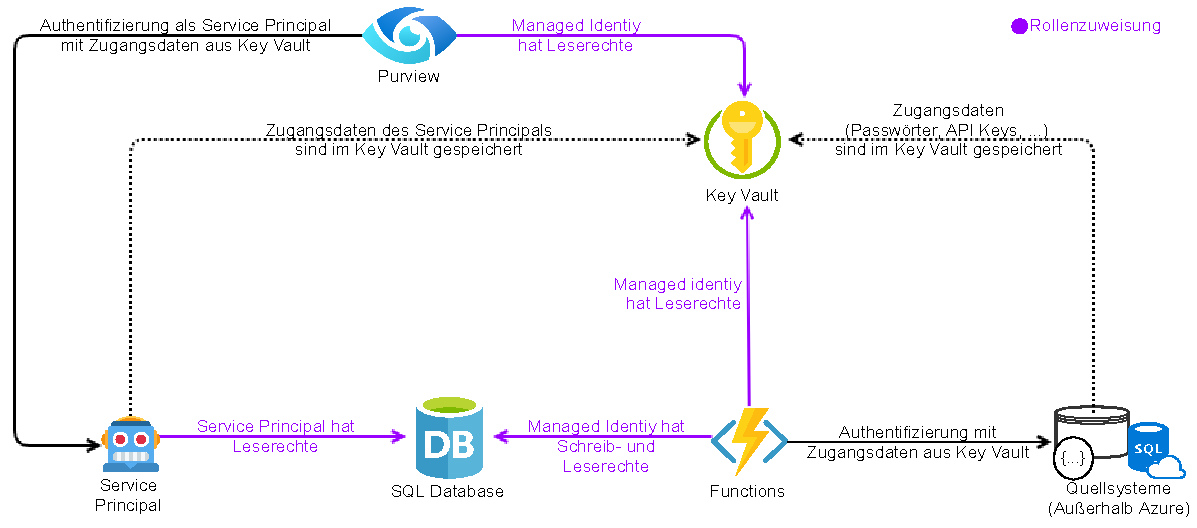
\includegraphics[width=\textwidth]{gfx/azure/res_auth.pdf}
 \caption[Authentifizierungskonzept für Ressourcen]{Authentifizierungskonzept für Ressourcen \cite[vgl.][]{riscutia_data_2021}}
\label{fig:chap04_ressourceAuth}
\end{figure}

% ================================================================================
\subsection{Netzwerkkommunikation} \label{subsec:infra:konfig:netzwerk}
Die Netzwerkeinstellungen der Ressourcen werden allgemein so eingerichtet, dass alles blockiert wird, dass nicht explizit zugelassen wurde. In den Firewall-Einstellungen des \textit{Key Vaults} werden \textit{Trusted Microsoft Services} erlaubt, da dies für \textit{Purview} erforderlich ist. Es handelt sich dabei um Azure Ressourcen, deren Code vollständig von Microsoft verwaltet wird. Fremde Azure Ressourcen, die benutzergenerierten Code ausführen, werden also weiterhin geblockt \cite[vgl.][]{msdoc_21_keyVault_netSec}.

Für den ausgehenden Datenverkehr der Funktionsapp soll eine statische IP-Adresse verwendet werden. Dafür wird im virtuellen Netzwerk ein neues Subnetz für die Funktionsapp und den dazugehörigen \textit{Storage Accounts} erstellt. In diesem Subnetz befindet sich ein \textit{NAT Gateway} mit einer zugewiesenen statischen IP-Adresse, welches den Datenverkehr weiterleitet. In den Konfigurationen der Funktionsapp wird erzwungen, dass alle Funktionen ihren ausgehenden Datenverkehr über dieses NAT Gateway leiten \cite[vgl.][]{msdoc_22_func_ip}. Diese IP-Adresse wird in den Firewall-Einstellungen des \ac{dwh}, des \textit{Key Vaults} und dem Cloud-Quellsystem zugelassen.

Für die Datenintegration aus einem on-premise Quellsystem wird ein Relay erstellt. Dem Relay wird eine \textit{Hybridverbindung} hinzugefügt, welche die Netzwerkadresse und den Port des lokalen Endpunkts definiert. Danach wird die \textit{Hybridverbindung} mit der Funktionsapp verknüpft. Nachdem die \textit{Hybridverbindung} in Azure bereitgestellt wurde, kann dort eine Gateway-Verbindungszeichenfolge entnommen werden. Damit erfolgt die manuelle Installation und Einrichtung der Anwendung \textit{Hybrid Connection Manager} auf dem on-premise Server. Die Kommunikation zwischen on-premise Server und Funktionsapp erfolgt nun über das Relay. Der \textit{Hybrid Connection Manager} verwendet ausschließlich den ausgehenden TCP Port 443, um sich mit dem Relay zu verbinden, weswegen keine Änderungen an der Firewall notwendig sind \cite[vgl.][]{msdoc_22_func_hybridConn}. Die Funktionsweise der Datenintegration über eine \textit{Hybridverbindung} wird in Abbildung~\ref{fig:chap04_hybridConn} dargestellt.

 \begin{figure}[htbp]
 \centering
 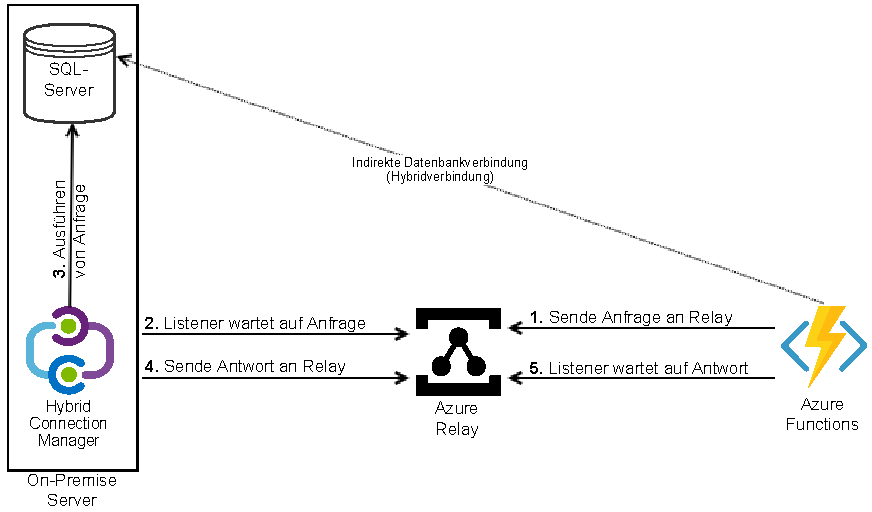
\includegraphics[width=\textwidth]{gfx/azure/hybridverbindung.pdf}
 \caption[Datenintegration über Hybridverbindung]{Funktionsweise der Datenintegration über eine Hybridverbindung: Die Datenbankverbindung von \textit{Functions} wird automatisch an das \textit{Relay} umgeleitet(1). Der \textit{Hybrid Connection Manager} erkennt die Anfrage über einen Listener(2) und führt sie auf der lokalen Datenbank aus(3). Die Antwort der Datenbank wird zurück an das \textit{Relay} gesendet(4). Ein Listener von \textit{Functions} sieht die Antwort und diese wird gelesen(5). \cite[vgl.][]{msdoc_22_func_hybridConn, msdoc_21_hybridConn_protocol}}
\label{fig:chap04_hybridConn}
\end{figure}

% ================================================================================
\subsection{Zugriff auf Datenquellen im virtuellen Netzwerk} \label{subsec:infra:konfig:vm}
Mit den bisherigen Netzwerkeinstellungen ist der Zugriff auf das \ac{dwh} nur für die Funktionsapp möglich. Um den Zugriff für Datenbankadministratoren und den Diensten \textit{Power BI} und \textit{Purview} zu ermöglichen, wird eine Windows~=\ac{vm} im gleichen virtuellen Netzwerk wie das \ac{dwh} bereitgestellt. Das Betriebssystem und die Daten der \ac{vm} werden auf einer virtuellen \textit{Premium SSD} Festplatte gespeichert. Diese befindet sich einem lokal redundanten Speichercontainer und wird dort, zum Schutz vor Verlust, mindestens dreimal repliziert. Daten, die sich in Ruhe befinden, werden auf der virtuellen Festplatte automatisch verschlüsselt. Jedoch gewährleistet Microsoft für eine einzelne \ac{vm}~=Instanz nicht die angeforderte Verfügbarkeit von 99,95\%. Aus diesem Grund wird eine zweite \ac{vm}~=Instanz in einer anderen Verfügbarkeitszone erstellt. Die Azure Region besteht aus drei getrennten Verfügbarkeitszonen, welche voneinander unabhängige Hardware verwenden. Dadurch ist sichergestellt, dass beim Ausfall eines Rechenzentrums immer noch eine weitere Instanz aktiv ist und die \ac{sla} liegt mit diesem Ansatz bei einer Verfügbarkeit von 99,99\% \cite[vgl.][]{soh_data_2020}. Um die Sicherheit zu optimieren, sollen die \acp{vm} keine öffentliche IP~=Adresse haben, damit der Zugriff nur innerhalb des virtuellen Netzwerks möglich ist. Der Dienst Bastion bietet für diesen Anwendungsfall, eine komfortable und sichere Möglichkeit über das Azure Portal im Webbrowser eine RDP~=Verbindung mit den \acp{vm} herzustellen. Bastion muss sich dazu in einem Subnetz innerhalb des gleichen virtuellen Netzwerks wie die \acp{vm} befinden \cite[vgl.][]{herath_azure_2022}.

Nachdem die gesamte Infrastruktur bereitgestellt wurde, kann über die \ac{vm}, der Zugriff für \textit{Power BI} und \textit{Purview} auf das \ac{dwh} ermöglicht werden. Die Funktionsweise des Verbindungsaufbaus zu den \acp{vm} ist analog zu der Hybridverbindung bei der Datenintegration, sodass kein eingehender Datenverkehr notwendig ist. Es muss keine \textit{Azure Relay} Ressource bereitgestellt werden, da dies beim Einrichten der Anwendungen im Hintergrund von Azure übernommen wird. Für \textit{Power BI} ist dazu die Anwendung \textit{On-premises Data Gateway} auf den \acp{vm} zu installieren. Dabei wird durch die Verwendung von zwei \acp{vm} ein \textit{Gateway Cluster} erzeugt, welches ein hochverfügbares Reporting ermöglicht. Nach der Einrichtung kann das \textit{Gateway Cluster} in \textit{Power BI} für Verbindungen verwendet werden \cite[vgl.][]{gunnarsson_pro_2020}. Für \textit{Purview} wird die Anwendung \textit{Self~=hosted Integration Runtime} gemäß Dokumentation installiert und eingerichtet \cite[vgl.][]{msdoc_22_purviewSHIR}. Auch hier wird das Aufsetzen von mehreren Instanzen für eine höhere Verfügbarkeit unterstützt \cite{msdoc_22_purviewSHIRHighAv}.

% ================================================================================
\subsection{Darstellung der vollständigen Infrastruktur} \label{subsec:infra:konfig:VollständigeInfrastruktur}
Die vollständige Infrastruktur, mit den in den letzten Abschnitten beschriebenen Details, wird in Abbildung~\ref{fig:chap04_VollständigeInfrastruktur} dargestellt.

 \begin{figure}[htbp]
 \centering
 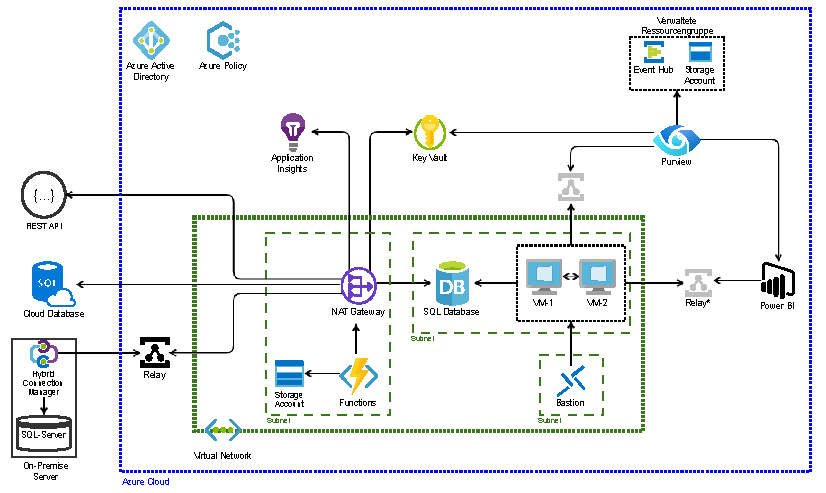
\includegraphics[width=\textwidth]{gfx/azure/infra.pdf}
 \caption[Vollständige Infrastruktur der Cloud BI]{Vollständige Infrastruktur der bereitgestellten Cloud BI}
 \caption*{\scriptsize{*Integraler Bestandteil von Power BI/Purview}}
\label{fig:chap04_VollständigeInfrastruktur}
\end{figure}